% Readable rewrite of the confidence-study 4-pager (MATH-AI 2026).
% Same claims, same numbers, same appendices as workshop_confidence.tex.
% Written as one argument: each section answers the objection the last one raised.
% Vocabulary: "represented" (a probe can read it) and "reported" (the model writes it).
% "Knowing" is scoped once in the introduction and never used as a claim.
%
% Build:  lualatex workshop_readable && bibtex workshop_readable && lualatex workshop_readable && lualatex workshop_readable
%

\documentclass{article}

\usepackage[dblblindworkshop,final,nonatbib]{style/neurips_2026}
\workshoptitle{The 6th Workshop on Mathematical Reasoning and AI}

% =============================================================
% Preamble — packages, macros, and authoring conventions for
% the GeoGen paper.  Include via % =============================================================
% Preamble — packages, macros, and authoring conventions for
% the GeoGen paper.  Include via % =============================================================
% Preamble — packages, macros, and authoring conventions for
% the GeoGen paper.  Include via \input{preamble} from geogen.tex.
% =============================================================

% --- core typography ---
% LuaLaTeX is natively UTF-8 and uses TU encoding; inputenc and fontenc are
% only needed under pdflatex. Wrap in \ifdefined for engine-portability.
\ifdefined\directlua\else
  \usepackage[utf8]{inputenc}
  \usepackage[T1]{fontenc}
\fi
\usepackage{microtype}
\usepackage{lmodern}

% --- math ---
\usepackage{amsmath, amssymb, amsthm}
\usepackage{mathtools}

% --- graphics, color, tables ---
\usepackage{graphicx}
\usepackage{subcaption}
\usepackage[dvipsnames,table]{xcolor}
\usepackage{float}
\usepackage{booktabs}
\usepackage{multirow}
\usepackage{array}
\usepackage{tabularx}
\usepackage{makecell}

% --- code listings ---
\usepackage{listings}
\lstset{
  basicstyle=\ttfamily\footnotesize,
  breaklines=true,
  showstringspaces=false,
  frame=single,
  framerule=0.4pt,
  rulecolor=\color{black!30},
  numbers=none,
}

% --- references ---
\usepackage[numbers,sort&compress]{natbib}
\usepackage{url}
\usepackage[hidelinks]{hyperref}
\usepackage[capitalize,noabbrev]{cleveref}

% --- diagrams (TikZ for figures we draw inline; pre-rendered figures use \includegraphics) ---
\usepackage{tikz}
\usetikzlibrary{positioning,arrows.meta,shapes.geometric,calc}

% --- misc ---
\usepackage{xspace}
\usepackage{enumitem}
\setlist[itemize]{itemsep=2pt, topsep=4pt}
\setlist[enumerate]{itemsep=2pt, topsep=4pt}

% =============================================================
% Project-specific macros
% =============================================================
% \GeoGen      = the methodology / pipeline (text -> TikZ -> SymPy -> verify)
% \GeoGenBench = the released benchmark (801 prompts + property lists)
% This paper is principally about the benchmark; the methodology is the means.
\newcommand{\GeoGen}{\textsc{GeoGen}\xspace}
\newcommand{\GeoGenBench}{\textsc{GeoGenBench}\xspace}
\newcommand{\geogen}{\GeoGen}              % alias
\newcommand{\geogenbench}{\GeoGenBench}    % alias

\newcommand{\strat}[1]{\textsf{#1}}        % strategy names (raw_code, structured)
\newcommand{\rawcode}{\strat{raw\_code}\xspace}
\newcommand{\structured}{\strat{structured}\xspace}

\newcommand{\modelname}[1]{\textsf{#1}}
\newcommand{\opus}{\modelname{Claude\,Opus\,4.7}\xspace}
\newcommand{\sonnet}{\modelname{Claude\,Sonnet\,4.6}\xspace}
\newcommand{\haiku}{\modelname{Claude\,Haiku\,4.5}\xspace}
\newcommand{\gpt}{\modelname{GPT-5.5}\xspace}
\newcommand{\geminipro}{\modelname{Gemini\,2.5\,Pro}\xspace}
\newcommand{\geminiflash}{\modelname{Gemini\,2.5\,Flash}\xspace}

\newcommand{\pp}{\,p.p.\xspace}            % percentage points
\newcommand{\dollars}[1]{\$#1}             % monetary

\newcommand{\true}{\textsc{true}\xspace}
\newcommand{\false}{\textsc{false}\xspace}

% Property type names (verbatim/typewriter)
\newcommand{\propname}[1]{\texttt{#1}}

% Tier shortcuts
\newcommand{\tone}{T1\xspace}
\newcommand{\ttwo}{T2\xspace}
\newcommand{\tthree}{T3\xspace}

% Editorial flags (visible in drafts; remove before camera-ready)
\newcommand{\TODO}[1]{{\color{red}\textbf{TODO:} #1}}
\newcommand{\NOTE}[1]{{\color{blue}\textit{[note: #1]}}}
\newcommand{\citationneeded}{{\color{red}[cite]}}
 from geogen.tex.
% =============================================================

% --- core typography ---
% LuaLaTeX is natively UTF-8 and uses TU encoding; inputenc and fontenc are
% only needed under pdflatex. Wrap in \ifdefined for engine-portability.
\ifdefined\directlua\else
  \usepackage[utf8]{inputenc}
  \usepackage[T1]{fontenc}
\fi
\usepackage{microtype}
\usepackage{lmodern}

% --- math ---
\usepackage{amsmath, amssymb, amsthm}
\usepackage{mathtools}

% --- graphics, color, tables ---
\usepackage{graphicx}
\usepackage{subcaption}
\usepackage[dvipsnames,table]{xcolor}
\usepackage{float}
\usepackage{booktabs}
\usepackage{multirow}
\usepackage{array}
\usepackage{tabularx}
\usepackage{makecell}

% --- code listings ---
\usepackage{listings}
\lstset{
  basicstyle=\ttfamily\footnotesize,
  breaklines=true,
  showstringspaces=false,
  frame=single,
  framerule=0.4pt,
  rulecolor=\color{black!30},
  numbers=none,
}

% --- references ---
\usepackage[numbers,sort&compress]{natbib}
\usepackage{url}
\usepackage[hidelinks]{hyperref}
\usepackage[capitalize,noabbrev]{cleveref}

% --- diagrams (TikZ for figures we draw inline; pre-rendered figures use \includegraphics) ---
\usepackage{tikz}
\usetikzlibrary{positioning,arrows.meta,shapes.geometric,calc}

% --- misc ---
\usepackage{xspace}
\usepackage{enumitem}
\setlist[itemize]{itemsep=2pt, topsep=4pt}
\setlist[enumerate]{itemsep=2pt, topsep=4pt}

% =============================================================
% Project-specific macros
% =============================================================
% \GeoGen      = the methodology / pipeline (text -> TikZ -> SymPy -> verify)
% \GeoGenBench = the released benchmark (801 prompts + property lists)
% This paper is principally about the benchmark; the methodology is the means.
\newcommand{\GeoGen}{\textsc{GeoGen}\xspace}
\newcommand{\GeoGenBench}{\textsc{GeoGenBench}\xspace}
\newcommand{\geogen}{\GeoGen}              % alias
\newcommand{\geogenbench}{\GeoGenBench}    % alias

\newcommand{\strat}[1]{\textsf{#1}}        % strategy names (raw_code, structured)
\newcommand{\rawcode}{\strat{raw\_code}\xspace}
\newcommand{\structured}{\strat{structured}\xspace}

\newcommand{\modelname}[1]{\textsf{#1}}
\newcommand{\opus}{\modelname{Claude\,Opus\,4.7}\xspace}
\newcommand{\sonnet}{\modelname{Claude\,Sonnet\,4.6}\xspace}
\newcommand{\haiku}{\modelname{Claude\,Haiku\,4.5}\xspace}
\newcommand{\gpt}{\modelname{GPT-5.5}\xspace}
\newcommand{\geminipro}{\modelname{Gemini\,2.5\,Pro}\xspace}
\newcommand{\geminiflash}{\modelname{Gemini\,2.5\,Flash}\xspace}

\newcommand{\pp}{\,p.p.\xspace}            % percentage points
\newcommand{\dollars}[1]{\$#1}             % monetary

\newcommand{\true}{\textsc{true}\xspace}
\newcommand{\false}{\textsc{false}\xspace}

% Property type names (verbatim/typewriter)
\newcommand{\propname}[1]{\texttt{#1}}

% Tier shortcuts
\newcommand{\tone}{T1\xspace}
\newcommand{\ttwo}{T2\xspace}
\newcommand{\tthree}{T3\xspace}

% Editorial flags (visible in drafts; remove before camera-ready)
\newcommand{\TODO}[1]{{\color{red}\textbf{TODO:} #1}}
\newcommand{\NOTE}[1]{{\color{blue}\textit{[note: #1]}}}
\newcommand{\citationneeded}{{\color{red}[cite]}}
 from geogen.tex.
% =============================================================

% --- core typography ---
% LuaLaTeX is natively UTF-8 and uses TU encoding; inputenc and fontenc are
% only needed under pdflatex. Wrap in \ifdefined for engine-portability.
\ifdefined\directlua\else
  \usepackage[utf8]{inputenc}
  \usepackage[T1]{fontenc}
\fi
\usepackage{microtype}
\usepackage{lmodern}

% --- math ---
\usepackage{amsmath, amssymb, amsthm}
\usepackage{mathtools}

% --- graphics, color, tables ---
\usepackage{graphicx}
\usepackage{subcaption}
\usepackage[dvipsnames,table]{xcolor}
\usepackage{float}
\usepackage{booktabs}
\usepackage{multirow}
\usepackage{array}
\usepackage{tabularx}
\usepackage{makecell}

% --- code listings ---
\usepackage{listings}
\lstset{
  basicstyle=\ttfamily\footnotesize,
  breaklines=true,
  showstringspaces=false,
  frame=single,
  framerule=0.4pt,
  rulecolor=\color{black!30},
  numbers=none,
}

% --- references ---
\usepackage[numbers,sort&compress]{natbib}
\usepackage{url}
\usepackage[hidelinks]{hyperref}
\usepackage[capitalize,noabbrev]{cleveref}

% --- diagrams (TikZ for figures we draw inline; pre-rendered figures use \includegraphics) ---
\usepackage{tikz}
\usetikzlibrary{positioning,arrows.meta,shapes.geometric,calc}

% --- misc ---
\usepackage{xspace}
\usepackage{enumitem}
\setlist[itemize]{itemsep=2pt, topsep=4pt}
\setlist[enumerate]{itemsep=2pt, topsep=4pt}

% =============================================================
% Project-specific macros
% =============================================================
% \GeoGen      = the methodology / pipeline (text -> TikZ -> SymPy -> verify)
% \GeoGenBench = the released benchmark (801 prompts + property lists)
% This paper is principally about the benchmark; the methodology is the means.
\newcommand{\GeoGen}{\textsc{GeoGen}\xspace}
\newcommand{\GeoGenBench}{\textsc{GeoGenBench}\xspace}
\newcommand{\geogen}{\GeoGen}              % alias
\newcommand{\geogenbench}{\GeoGenBench}    % alias

\newcommand{\strat}[1]{\textsf{#1}}        % strategy names (raw_code, structured)
\newcommand{\rawcode}{\strat{raw\_code}\xspace}
\newcommand{\structured}{\strat{structured}\xspace}

\newcommand{\modelname}[1]{\textsf{#1}}
\newcommand{\opus}{\modelname{Claude\,Opus\,4.7}\xspace}
\newcommand{\sonnet}{\modelname{Claude\,Sonnet\,4.6}\xspace}
\newcommand{\haiku}{\modelname{Claude\,Haiku\,4.5}\xspace}
\newcommand{\gpt}{\modelname{GPT-5.5}\xspace}
\newcommand{\geminipro}{\modelname{Gemini\,2.5\,Pro}\xspace}
\newcommand{\geminiflash}{\modelname{Gemini\,2.5\,Flash}\xspace}

\newcommand{\pp}{\,p.p.\xspace}            % percentage points
\newcommand{\dollars}[1]{\$#1}             % monetary

\newcommand{\true}{\textsc{true}\xspace}
\newcommand{\false}{\textsc{false}\xspace}

% Property type names (verbatim/typewriter)
\newcommand{\propname}[1]{\texttt{#1}}

% Tier shortcuts
\newcommand{\tone}{T1\xspace}
\newcommand{\ttwo}{T2\xspace}
\newcommand{\tthree}{T3\xspace}

% Editorial flags (visible in drafts; remove before camera-ready)
\newcommand{\TODO}[1]{{\color{red}\textbf{TODO:} #1}}
\newcommand{\NOTE}[1]{{\color{blue}\textit{[note: #1]}}}
\newcommand{\citationneeded}{{\color{red}[cite]}}


\title{Knowing Before Saying: Internal Correctness Signals in Mathematical Reasoning}

\author{%
  Mei Chen$^{1}$ \quad Gordon Stein$^{1}$ \quad Andreas Ziegler$^{2}$ \\
  $^{1}$Renaissance Philanthropy \quad
  $^{2}$Institute for Aerospace Studies, University of Toronto \\
  {\small\texttt{\{mei.chen, gordon.stein\}@renphil.org} \quad \texttt{andreas.ziegler@robotics.utias.utoronto.ca}}
}

\begin{document}

\maketitle

\begin{abstract}
Language models are often confidently wrong.
We ask whether a model's activations carry a better signal of its own errors than its stated confidence does.
We test four open models on four tasks: MMLU-Pro, MATH, GPQA-Diamond, and a geometry task graded by a compiler.
We put a linear probe on the hidden state to predict whether an answer is right.
This probe was better than the model's stated confidence in 12 of 16 cases, by 0.09 AUROC on average.
The gap is largest on MATH.
The probe is not just detecting hard questions: it still works when the same question is attempted five times.
On Mistral and MMLU-Pro, the signal exists before the model is asked how confident it is.
On Mistral, the model uses this signal when it reports confidence.
When we erase the signal from the hidden state, the stated confidence no longer separates right answers from wrong ($0.84 \to 0.56$), while erasing a random direction did nothing.
On GLM, erasing it changes nothing.
On Qwen3.6 the stated confidence carries almost nothing to erase, and amplifying the signal adds a little.
In short, four open models carry more confidence signal about their own errors than they report.
In Mistral, we have shown this direction is used when it self-reports confidence.
\end{abstract}

\section{Introduction}
\label{sec:intro}

A language model that is confidently wrong is a problem.
Its stated confidence, which we call its self-report, is a signal for deciding whether to trust its answer or not.
This paper asks whether the model's activations contain a signal related to its confidence.

We have two hypotheses for a model that gives a wrong answer with high confidence.
The first is that the model has no internal signal that it might be wrong.
It is blindly confident, and this is a capability problem.
The second is that the model's activations hold an error signal, but the signal does not reach its self-report.
The latter is a reporting problem.

In this paper we tell these two apart.
We read the model's hidden state with a linear \emph{probe} and compare what the probe finds to what the model reports.
We say a fact is \emph{represented} when a probe can read that fact from the model's state.
We say a fact is \emph{reported} when that fact reaches the confidence number the model writes.
We refer to \emph{knowing} as shorthand for a representation used by self-report.
We make no claim about awareness.
A probe alone could not support one.

Prior work reads the truth of a statement from activations~\citep{azaria2023internal, burns2023discovering, marks2024geometry}, and reads a model's own errors from its hidden state better than its output reveals them~\citep{orgad2025llms, chwang2024androids}.
A model's output probabilities are often better calibrated than its words~\citep{kadavath2022language}, and asked confidence is known to be overconfident~\citep{lin2022teaching, tian2023just, xiong2024can}.
Training on a model's own self-assessments can narrow that gap~\citep{liu2026rlmf}.
Probes can latch onto confounds rather than the intended variable~\citep{levinstein2024still}.
Intervening on a truth direction changes what a model says~\citep{li2023iti, zou2023representation}.
We apply those tools to the model's own attempts, and then ask whether the self-report depends on the representation.

\section{Reading the state}
\label{sec:reading}

\paragraph{Models and tasks.}
We test four open models of three architectures: Mistral-Small-24B (dense), Qwen3.6-27B (gated linear attention interleaved with full attention), and GLM-4.7-Flash and Gemma-4-26B (mixture of experts).
Qwen3.6 and GLM are hybrid reasoners: they answer with thinking on and report confidence with thinking off (\cref{app:checkpoints}).
Each answers 150 questions, five times each, on MMLU-Pro~\citep{wang2024mmlupro}, MATH~\citep{hendrycks2021math}, and GPQA-Diamond~\citep{rein2023gpqa}, and 91 geometry construction prompts, four times each, graded by the GeoGenBench compiler~\citep{chen2026geogenbench}.
The 150 are a seeded random draw from each test set; MATH uses the 500-problem test subset at all levels.
Multiple choice is graded by letter match, MATH by symbolic equivalence of the boxed answer, and geometry by whether the construction compiles and passes its checks.
Attempts are sampled at temperature 0.8 (\cref{app:checkpoints}).
Four models times four tasks gives 16 cells: 750 attempts each, or 364 for geometry.

\paragraph{Three-step prompting structure.}

\begin{enumerate}[nosep,leftmargin=1.4em]
  \item The model is shown the question and asked to write, before answering, a number from 0 to 100 for how confident it is that it will get it right.
  \item It is then asked to answer the question.
  \item It is asked to write, again as a number from 0 to 100, how confident it is that the answer it just gave is correct.
\end{enumerate}

\paragraph{The probe.}
At the moment the model is about to write its confidence digit in step 3, after the attempt, we record the number and the residual-stream hidden state at that token (2,048 to 5,120 dimensions, depending on the model).
Three other read sites appear below and are listed in \cref{app:sites}: the step-1 digit, the last token of the bare question, and the last token of the answer.
The probe is a linear classifier on that vector: features are standardized, reduced to 50 principal components, and fed to an L2-regularized logistic regression that predicts whether the attempt was correct.
We fit it with five-fold cross-validation grouped by question, so all attempts at a question fall in the same fold and the probe is always scored on questions it never saw; the standardization and the PCA are fit inside each training fold, so no held-out record touches them.
The read depth is fixed in advance at 70\% of the network (\cref{app:checkpoints}, \cref{fig:layers}).
Every readout is scored with AUROC.

\begin{figure}[t]
\centering
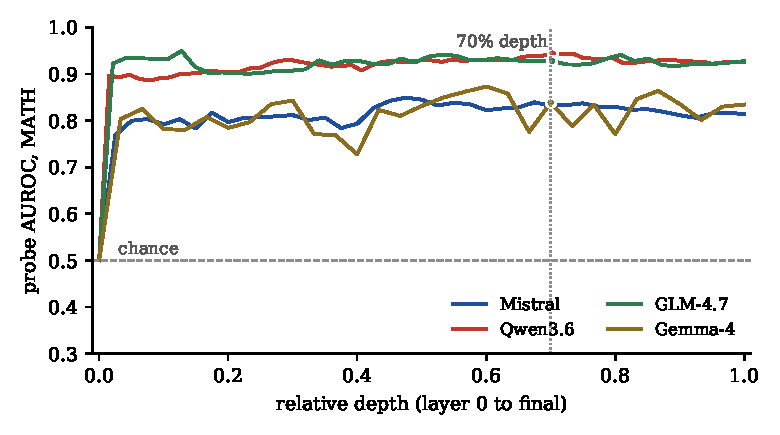
\includegraphics[width=0.46\linewidth]{figures/layer_curve_math.pdf}
\caption{Probe AUROC by depth on MATH, four models, grouped five-fold, mean over folds. Layer 0 reads 0.500 because its token is identical in every record. The dot is the fixed 70\% layer; the best layer beats it by at most 0.04.}
\label{fig:layers}
\end{figure}

\paragraph{The activation state carries more than self-report.}
The probe beats the model's self-report in \textbf{12 of 16} cells, with one tie.
The mean gain is $+0.09$ AUROC (\cref{app:cells}).
The gap is largest on MATH, $+0.20$ averaged over the four models.
Mistral on MATH is the running example below because it is the cell we intervene on in \cref{sec:causal}, not because its gap is large: at $+0.04$ it is the smallest MATH gap.
The model is never told whether it got the answer right.
Yet after attempting, it raises its confidence, and it raises it more on the attempts it got wrong ($+22$ points) than on the ones it got right ($+16$ points).
The probe on the same records reads 0.83.
The state tracks correctness better than the self-report does.

\paragraph{Why MATH.}
On MATH, right and wrong answers have the same shape.
Both are a chain of steps ending in a boxed result, so the model cannot tell from the look of its answer whether it went wrong.
\cref{app:worked} follows one attempt where a single wrong subtraction leads to a wrong answer, and the model then raises its confidence.
Shape still carries a little signal.
A baseline classifier that sees only surface features of the answer text, such as its length and line count, reaches 0.74, but the probe reaches 0.83.
Geometry is the opposite case.
A failed construction usually does not compile, so the failure is visible in the answer itself, and there the surface baseline does as well as the probe.
The internal signal helps most where the failure is invisible from outside.

\paragraph{Controls.}
Three things could make a probe look better than it is; the next section tests each.
It could be reading how hard the question is rather than the attempt, so we compare attempts within one question.
It could be reading the shape of the output, so we compare it with the surface baseline in every cell; on Mistral, adding the probe to the surface features raises AUROC by $+0.21$ on MMLU-Pro, $+0.07$ on MATH, and $+0.05$ on GPQA, and lowers it by $0.11$ on geometry, where the combined classifier overfits 364 records.
And it could be reading something that was there before the attempt, so we read the state before the attempt as well.
As a sanity check on the pipeline, not a control, we also read the input layer, where the token is identical in every record and the probe sits at exactly 0.5 by construction.
These controls were run on Mistral only, for time.
Its four cells reproduce the headline.

\section{What the signal is}
\label{sec:what}

\paragraph{Difficulty control.}
A probe that beats self-report could be doing something simpler.
It could be learning which questions are hard.
Hard questions fail more often, so a difficulty detector would predict correctness without reading the attempt.
We run two checks to investigate this.

First, hold the question fixed.
Each question is attempted five times, so within one question, difficulty cannot vary.
On Qwen3.6 and GLM on MMLU-Pro, the probe still separates the successful attempts from the failed ones (0.74 and 0.73), while the model's own P(True), its probability of answering ``True'' when asked whether it was right, drops to near chance (0.47 and 0.59).
On Mistral on MATH the picture is different: within a question the probe reads 0.63 and stated confidence 0.65, so in that cell, the probe beats self-report only when comparing across different questions, likely by detecting question difficulty, but not when comparing the five attempts at a single question, where difficulty is held constant (\cref{app:cells}).

Second, ask when the direction appears.
Before the attempt, all five tries at a question look identical to the model.
Anything readable at that moment is about the question, not the attempt.
A difficulty detector would still work there.
Our probe, trained on the state after the attempt, reads 0.49 at that pre-attempt point on MMLU-Pro, which is chance, against 0.75 at the post-attempt token where it was trained.
However, this drop could partly reflect the mismatch in token position between training and testing, rather than a true absence of difficulty information, which is why the within-question test, which avoids that mismatch, is the more reliable of the two controls.
Geometry is the exception.
There the pre-attempt state already predicts failure, so that cell is mostly difficulty.
GPQA is the other weak cell: Mistral is near chance on it, so the labels are partly luck, and nothing reads above 0.6 at any site.

\paragraph{Reading before the question.}
A subtler worry.
Every read so far came after the model was asked to assess itself.
Maybe the question creates the signal rather than reveals it.
So we read the state at the last token of the answer, before any confidence question exists.
This test can only work where the question alone predicts nothing.
That rules out MATH, where the question alone already predicts correctness at 0.79, and GPQA, where nothing is readable at any site.
On MMLU-Pro the question alone reads 0.57, chance.
At the end of the answer, correctness reads 0.69.
Asking the model to self-assess sharpens it to 0.77.
So the signal does not depend on our confidence prompt; the prompt only sharpens it.

\paragraph{Transfer across domains.}
\cref{tab:transfer} trains a probe on one domain and tests it on each of the others.
On Mistral it keeps about 90\% of its lift above chance (0.69 off the diagonal against 0.71 on it).
The full four-model matrix showed the same pattern.
The one exception is Gemma-4, where probes trained on geometry do not transfer out, though probes trained elsewhere transfer in.

\begin{table}[t]
\caption{Mistral, probe AUROC against the external grade. Rows: training domain; columns: test domain; bold: in-domain.}
\label{tab:transfer}
\centering
\small
\begin{tabular}{lcccc}
\toprule
\textbf{train $\downarrow$ test $\rightarrow$} & \textbf{GeoGen} & \textbf{MMLU-Pro} & \textbf{MATH} & \textbf{GPQA} \\
\midrule
GeoGen & \textbf{0.68} & 0.67 & 0.78 & 0.56 \\
MMLU-Pro & 0.70 & \textbf{0.75} & 0.84 & 0.59 \\
MATH & 0.80 & 0.72 & \textbf{0.83} & 0.57 \\
GPQA & 0.60 & 0.69 & 0.74 & \textbf{0.57} \\
\bottomrule
\end{tabular}
\end{table}

\section{Whether self-report depends on the residual signal}
\label{sec:causal}

\paragraph{Erasing and amplifying the signal direction.}
A model could carry a perfect internal record of its errors and never consult it during self-report.
The only way to find out is to change the record and watch the number.
At the confidence token, after the answer is written so the answer cannot change, we scale the model's position along the correctness direction by a gain $g$.
Gain 1 leaves the model untouched, gain 0 erases the per-attempt information, and gains 2 and 4 exaggerate it.
We run this on Mistral and MATH, 150 held-out records, with a random direction of the same norm as a control; \cref{app:intervention} gives the exact transformation.
The confidence turn is regenerated greedily at each setting, so the untouched self-report here (0.84) is not the sampled self-report of \cref{app:cells} (0.79) on the same cell.
\cref{tab:ablation} shows what the model wrote at each setting.

\begin{table}[t]
\caption{Mistral on MATH, 150 held-out records; AUROC is that of the stated confidence against the external grade. The correctness direction scaled by a gain at the confidence token, after the answer is written. Bold marks the erased and quadrupled settings; unparseable means the output no longer parsed as a confidence.}
\label{tab:ablation}
\centering
\small
\begin{tabular}{lcccc}
\toprule
 & \textbf{untouched} & \textbf{erased} & \textbf{doubled} & \textbf{quadrupled} \\
gain on the correctness direction & 1 & 0 & 2 & 4 \\
\midrule
mean confidence, wrong / right answers & 84 / 96 & \textbf{97 / 98} & 70 / 94 & \textbf{54 / 88} \\
AUROC of self-report & 0.84 & \textbf{0.56} & 0.85 & 0.82 \\
same, with a random direction & 0.84 & 0.83 & 0.84 & unparseable \\
\bottomrule
\end{tabular}
\end{table}

\paragraph{Result on Mistral.}
Self-report loses its information when the signal direction is erased.
Its AUROC falls from 0.84 to 0.56, a drop of 0.27 before rounding (95\% interval 0.12 to 0.42).
Part of the drop is ties at the ceiling: 89 of the 150 erased confidences are 97 or above, against 61 untouched.
Erase a random direction and nothing happens.
This is not generic damage.
The output stays well formed.
Confidence on wrong answers goes \emph{up} to match right answers, so the model becomes uniformly sure rather than confused.
Amplify the direction and the opposite happens: confidence on wrong answers falls while right answers hold, and the expected calibration error halves, $0.34 \to 0.19$ on these 150 greedy records (the 750-record ECE in \cref{app:stats} is 0.27).
Two checks say the effect is specific.
The same intervention at 30\% of the way through the network does nothing.
A direction learned on MMLU-Pro, where surface features cannot explain the probe, still controls the MATH report ($0.88 \to 0.71$, on a different held-out 150).

\paragraph{Results on GLM and Qwen3.6.}
GLM has the strongest signal in the study: within a question on MATH, the probe reads 0.87 while the model's own P(True) reads 0.53 (matrix capture; the steering uses a fresh capture of the cell, \cref{app:checkpoints}).
Yet erasing the direction leaves self-report where it was, 0.76 before and after.
That bounds how much the report uses this direction at this layer; a redundant encoding elsewhere could still feed it.
Qwen3.6 is a third case.
Its self-report on MATH is nearly uninformative to begin with (AUROC 0.54; it writes 97 or 98 on right and wrong answers alike), so erasing the direction has nothing to remove.
Amplifying the direction fourfold raises the self-report's AUROC to 0.63, while a random direction leaves it at 0.54.
Both models represent their errors and report them poorly.
These are our cleanest cases of represented but not reported, and they make the causal result a fact about particular models, not models in general.

\section{The Jacobian lens}
\label{sec:lens}

\paragraph{A label-free check.}
A trained probe might have overfit to our data.
So we add an instrument that uses no correctness labels.
We fit the Jacobian lens~\citep{gurnee2026workspace} on generic text.
It reads an activation for what it pushes the model to say next.
We score each state by how far it leans toward ``wrong'' over ``correct.''
On dense models the lens matches the probe.
On Mistral it reads 0.82 on MATH and 0.75 on MMLU-Pro, against the probe's 0.83 and 0.75, and it reads 0.5 at the input layer, as it must, since that token is identical in every record.
Two instruments built from different evidence find the same direction.
And because the lens reads through the model's own output pathway, that direction sits where it could influence what the model says.

\paragraph{Where the lens fails.}
The lens is a fixed dictionary from hidden-state directions to words, built once from generic text.
On a dense model one dictionary is enough, because every input takes the same path to the output.
GLM routes each input through a different subset of experts, and Qwen3.6 mixes two kinds of attention layers, so there is no single path and the lens averages many into a blur.
The numbers show it: on GLM the lens's entries for ``correct'' and ``wrong'' point almost the same way, cosine 0.96, against 0.40 on a dense model.
On GLM the lens scores 0.31, below chance.
This happens because the lens has found the right direction in the hidden state but cannot tell which end of it means ``correct'' and which means ``wrong''; it has lost the sign of the direction.
This is exactly what the 0.96 cosine similarity between the ``correct'' and ``wrong'' vectors predicts.
On Qwen3.6 the lens scores 0.43, while the probe still works on both models.
Swap Qwen3.6 for Qwen2.5-14B, same family but dense, and the lens jumps to 0.88.
The swap also changes size and training recipe, so it is a quasi-control, not an isolation.
The signal is there in every model.
The lens can read it only on dense models, where every input follows the same path from hidden state to output, so a single fixed dictionary fits them all.

\section{What this means}
\label{sec:discussion}

\paragraph{Practical use.}
Without an exact checker, the probe beats stated confidence in 12 of 16 cells.
Against two label-free readouts it is closer: P(True) and the mean log-probability of the answer beat stated confidence in every cell where we have them, and on Gemma and MATH both beat the probe (\cref{app:cells}).
The probe's advantage is largest exactly where the model's confidence is useless.

\paragraph{Limitations.}
A probe could be reading properties of failed output rather than a self-assessment.
The surface baseline bounds this without closing it, most loosely on MATH, geometry (\cref{app:alternatives}), and GLM.
Every number is a single seed.
The causal result holds on Mistral.
On GLM erasing one direction at one layer does nothing, which does not rule out a redundant encoding elsewhere; on Qwen3.6 the self-report is too uninformative for erasing to test, though amplifying moves it.
Gemma-4 leaves too few failures to test.
Two of the four tasks are not mathematical.
Within a question, the probe's lead over self-report on Mistral and MATH disappears.
A base model could tell us whether preference tuning created the gap between represented and reported.

\paragraph{Takeaway.}
Four open models carry information about their own errors that their self-report does not.
In Mistral, we have shown it is used when it self-reports.
In one, erasing it changes nothing.
In one, there is nothing to erase.

\bibliographystyle{plainnat}
\bibliography{refs,refs_confidence}

\appendix
\crefalias{section}{appendix}
\crefname{appendix}{Appendix}{Appendices}
\Crefname{appendix}{Appendix}{Appendices}
\section{The elicitation protocol, and one record end to end}
\label{app:worked}

This appendix gives the exact prompts behind every record, then one complete record
from the Mistral-Small-24B $\times$ MATH cell, summarized first and then given in full.

\begin{center}
\footnotesize
\fbox{\begin{minipage}{0.96\linewidth}
\textbf{One record, Mistral-Small-24B $\times$ MATH.} \emph{What integer $n$ satisfies $0\le n<18$ and $n\equiv -11213141 \pmod{18}$?}
The model sets the problem up correctly and gets $18\times622953 = 11213154$ right, then writes $r = -11213141 + 11213154 = 3$ and answers $3$.
That subtraction gives $13$, which is the gold answer.
Stated confidence: $90$ before the attempt, $95$ after it.
Other readouts of the same attempt: P(True), the probability the model assigns to ``True'' when asked whether its answer is correct, $0.32$; mean answer log-probability $-0.05$.
\end{minipage}}
\end{center}

\noindent
A single arithmetic slip inside a fluent derivation. Having just made the error, the model
revises its stated confidence upward, while P(True) on the same transcript assigns only
0.32 probability to correctness. The rest of this appendix gives the prompts and the full transcript.

\subsection{Prompts}

Each record is four forward passes: the three turns of \cref{sec:reading} plus one read taken
beforehand, at the last prompt token of the bare question, before any elicitation. The confidence turns
run with thinking off so the read lands on a clean one-line reply; the attempt turn runs
with thinking on for hybrid reasoners. The fixed \texttt{Confidence: N} format is what makes
the read site content-neutral: the digit token has identical local context on every record,
so layer-0 activations carry no signal by construction.

\paragraph{System prompt (MATH).}
\begin{quote}\ttfamily\footnotesize
Solve the problem step by step. Put your final answer in \textbackslash boxed\{\}.
\end{quote}

\paragraph{Turn 1, prospective confidence.} The problem is followed by:
\begin{quote}\ttfamily\footnotesize
Before answering, estimate how likely you are to answer this question correctly. Reply with EXACTLY one line and nothing else:\\
Confidence: N\\
where N is an integer from 0 (certain to be wrong) to 100 (certain to be correct). Do NOT answer yet.
\end{quote}

\paragraph{Turn 2, the attempt.} The turn-1 reply is left in context as the assistant message, then:
\begin{quote}\ttfamily\footnotesize
Now give your final answer inside \textbackslash boxed\{\}.
\end{quote}

\paragraph{Turn 3, retrospective confidence.} The attempt is left in context, then:
\begin{quote}\ttfamily\footnotesize
Now assess the answer you just gave. On a scale of 0 to 100, how confident are you that it is correct? Reply with exactly one line and nothing else:\\
Confidence: N
\end{quote}

\paragraph{P(True) baseline.} A separate teacher-forced branch off turn 2, no generation.
Next-token mass on \texttt{True} versus \texttt{False}:
\begin{quote}\ttfamily\footnotesize
Consider your final answer above. Is it correct? Reply with exactly one word: True or False.
\end{quote}

Grading is external and is never shown to the model, so the turn-3 revision is blind
self-assessment.

\subsection{Read sites}
\label{app:sites}
Four positions in the three-turn exchange are read in the paper. Each is the residual-stream state at one token, at 70\% of depth unless stated.

\begin{table}[H]
\centering\small
\begin{tabular}{@{}lp{0.46\linewidth}p{0.36\linewidth}@{}}
\toprule
\textbf{site} & \textbf{token} & \textbf{used in} \\
\midrule
prompt & last token of the bare question, before turn 1 & ``question alone'' reads, \cref{sec:what} \\
pre & the confidence digit of turn 1, before the attempt & ``pre'' column of \cref{tab:knowing} \\
answer & last token of the turn-2 answer, before any confidence question & ``reading before the question,'' \cref{sec:what} \\
post & the confidence digit of turn 3, after the attempt & the probe, the lens, the intervention; every number not marked otherwise \\
\bottomrule
\end{tabular}
\end{table}

\subsection{One record, verbatim}

Record \texttt{math\_test\_number\_theory\_753}, sample 2 of 5.

\paragraph{Problem.} \emph{What integer $n$ satisfies $0 \le n < 18$ and $n \equiv -11213141 \pmod{18}$?}

\paragraph{Turn 1 reply.} \texttt{Confidence: 90}

\paragraph{Turn 2 reply (complete).}
\begin{quote}\footnotesize
First, we need to find the remainder when $-11213141$ is divided by $18$.

1. Calculate $-11213141 \bmod 18$:
\[ -11213141 \div 18 \approx -622952.2778 \]
The integer part of the division is $-622953$.
\[ -11213141 = 18 \times (-622953) + r \]
where $r$ is the remainder.

2. Calculate the remainder $r$:
\[ r = -11213141 - 18 \times (-622953) \]
\[ r = -11213141 + 11213154 \]
\[ r = 3 \]

Therefore,
\[ -11213141 \equiv 3 \pmod{18} \]

So, the integer $n$ that satisfies $0 \le n < 18$ and $n \equiv -11213141 \pmod{18}$ is $3$.
\end{quote}

\paragraph{Turn 3 reply.} \texttt{Confidence: 95}

\paragraph{What happened.}
The method is right and every intermediate is right: $18 \times 622953 = 11213154$ checks out,
and the model has written the correct subtraction on the line above its answer.
It then evaluates $-11213141 + 11213154$ as $3$ rather than $13$. Gold is $13$.
Nothing in the presentation marks the slip. The derivation is well formed, correctly
structured, and confidently laid out, which is precisely why stated confidence rises
from $90$ to $95$ across an attempt that failed.

\paragraph{Readouts of this attempt.}
\begin{center}
\small
\begin{tabular}{lc}
\toprule
\textbf{readout} & \textbf{value} \\
\midrule
stated confidence, prospective (turn 1) & 90 \\
stated confidence, retrospective (turn 3) & 95 \\
P(True) & 0.32 \\
mean answer log-probability & $-0.05$ \\
\midrule
graded outcome & \textbf{incorrect} \\
\bottomrule
\end{tabular}
\end{center}

\noindent
This is one record, chosen to illustrate the failure mode rather than to carry evidential
weight; representative cell-level numbers are in \cref{tab:knowing}, \cref{app:cells}.

\section{Calibration beyond ECE, and cell-level multiplicity}
\label{app:stats}

ECE depends on binning and on sample composition, so we report two binning-free proper
scoring rules alongside it. On Mistral $\times$ MATH (750 records, accuracy 0.648), the
model's retrospective stated confidence gives Brier $0.262$ and NLL $1.470$ against a
10-bin ECE of $0.271$. P(True) on the same records gives Brier $0.386$: better ordered
than stated confidence, worse calibrated in absolute terms. The steering results in
\cref{tab:ablation} are reported as ECE because the steered runs stored per-gain
aggregates rather than per-record confidences; recomputing Brier and NLL at each gain
requires re-running the intervention and is the first thing we would add.

The cell-level bootstrap counts in \cref{tab:knowing} are uncorrected. With 16 cells,
some individually significant results are expected under the null, so the cell counts
should be read as descriptive. The aggregate pattern is the claim that carries weight:
the effect is positive in 12 of 16 cells with one tie, significantly positive in 10,
and never significantly negative. A
hierarchical model pooling across cells with model and domain as random effects is the
right test and is not yet run.

\section{Alternative explanations for the probe signal}
\label{app:alternatives}
A probe could key on properties of failed derivations rather than on a dedicated
metacognitive variable: low token probability, hedging language, or, on MATH, an
early-layer channel next to the answer text. Our surface-features baseline (answer
length, digit count, line count, word count, brace count) bounds this without closing
it, and the bound is domain dependent: adding the probe to the surface features raises
AUROC by $+0.21$ on MMLU-Pro but only $+0.07$ on MATH and $-0.11$ on geometry, where a
construction that fails to compile is visibly malformed. Two results argue against a pure surface account on the
domains where the signal is strong. A direction fitted on MMLU-Pro, where surface
reaches only 0.54 against a probe of 0.75, still governs MATH's self-report under
ablation ($0.880 \to 0.709$). And the pre-attempt read, taken where the activation is
byte-identical across a question's attempts, cannot recover the post-attempt direction
on MMLU-Pro (0.490, chance), which a surface-of-the-question account would predict it
could. A linear probe at one token also undercounts nonlinear or multi-token signal, so
the reported numbers are a floor.

\section{Per-cell numbers and specificity controls}
\label{app:cells}
\begin{table}[H]
\caption{All 16 cells, post-attempt, AUROC against the external grade: stated confidence / probe at the fixed 70\% layer, bold marks the larger. The probe wins 12, ties 1 (Mistral $\times$ GPQA) and loses 3; mean gap $+0.10$; MATH mean gap $+0.20$. A paired bootstrap is significantly positive in 10 of 16 and never significantly negative, uncorrected at the cell level (\cref{app:stats}).}
\label{tab:cells}
\centering\small
\begin{tabular}{@{}lcccc@{}}
\toprule
\textbf{stated / probe} & \textbf{MMLU-Pro} & \textbf{MATH} & \textbf{GPQA} & \textbf{Geometry} \\
\midrule
Gemma-4 & \textbf{0.76} / 0.74 & 0.57 / \textbf{0.75} & \textbf{0.80} / 0.75 & 0.66 / \textbf{0.71} \\
Qwen3.6 & 0.74 / \textbf{0.75} & 0.59 / \textbf{0.90} & 0.61 / \textbf{0.81} & \textbf{0.87} / 0.70 \\
GLM & 0.67 / \textbf{0.85} & 0.70 / \textbf{0.95} & 0.54 / \textbf{0.70} & 0.66 / \textbf{0.95} \\
Mistral & 0.67 / \textbf{0.74} & 0.79 / \textbf{0.83} & 0.57 / 0.57 & 0.65 / \textbf{0.80} \\
\bottomrule
\end{tabular}
\end{table}

\begin{table}[H]
\caption{Label-free baselines and within-question numbers on the seven cells whose records we hold (\cref{app:checkpoints}). Pooled: AUROC over all attempts. Within: mean AUROC over questions with both outcomes ($n$ in the second column). P(True) is the model's probability of answering ``True'' when asked whether its answer was right; log-prob is the mean token log-probability of the answer. Within-question probe values are available for the Mistral cells only; the probe here is the matrix-capture probe of \cref{tab:cells}. Gemma-4 $\times$ MATH has four mixed questions, so its within-question values are not meaningful and are omitted.}
\label{tab:baselines}
\centering\scriptsize\setlength{\tabcolsep}{3.5pt}
\begin{tabular}{@{}lccccccccc@{}}
\toprule
 & & \multicolumn{4}{c}{\textbf{pooled}} & \multicolumn{3}{c}{\textbf{within question}} \\
\cmidrule(lr){3-6}\cmidrule(lr){7-9}
\textbf{cell} & \textbf{acc. / mixed} & \textbf{stated} & \textbf{P(True)} & \textbf{log-prob} & \textbf{probe} & \textbf{stated} & \textbf{P(True)} & \textbf{probe} \\
\midrule
Mistral $\times$ MMLU-Pro & 0.64 / 66 & 0.67 & 0.71 & \textbf{0.72} & \textbf{0.74} & 0.65 & 0.69 & \textbf{0.72} \\
Mistral $\times$ MATH & 0.65 / 54 & 0.78 & 0.77 & 0.72 & \textbf{0.83} & \textbf{0.65} & 0.55 & 0.63 \\
Mistral $\times$ GPQA & 0.44 / 91 & 0.57 & \textbf{0.61} & 0.56 & 0.57 & 0.53 & \textbf{0.63} & 0.55 \\
Mistral $\times$ Geometry & 0.10 / 20 & 0.62 & -- & -- & \textbf{0.80} & 0.36 & -- & \textbf{0.62} \\
GLM $\times$ MATH & 0.71 / 54 & 0.73 & 0.74 & 0.66 & \textbf{0.95} & 0.53 & \textbf{0.62} & -- \\
Qwen3.6 $\times$ MATH & 0.48 / 88 & 0.59 & 0.86 & 0.70 & \textbf{0.90} & 0.50 & \textbf{0.77} & -- \\
Gemma-4 $\times$ MATH & 0.94 / 4 & 0.60 & \textbf{0.82} & 0.78 & 0.75 & -- & -- & -- \\
\bottomrule
\end{tabular}
\end{table}

\begin{table}[H]
\caption{Mistral specificity controls (AUROC). ``pre'' is the last prompt token before the attempt; ``post'' is after the attempt; ``resid.'' removes the pre score; ``post$\to$pre'' applies the fitted post readout at the pre-attempt site, where only difficulty is visible. Within-question comparisons for Qwen3.6 and GLM on MMLU-Pro from the matrix capture: probe 0.74 and 0.73 against P(True) 0.47 and 0.59.}
\label{tab:knowing}
\centering\small
\begin{tabular}{@{}lcccc@{}}
\toprule
\textbf{Mistral} & \textbf{pre} & \textbf{post} & \textbf{resid.} & \textbf{post$\to$pre} \\
\midrule
MMLU-Pro & 0.568 & 0.754 & 0.751 & 0.490 \\
MATH & 0.792 & 0.834 & 0.701 & 0.624 \\
GPQA & 0.593 & 0.572 & 0.544 & 0.479 \\
GeoGen & 0.770 & 0.676 & 0.505 & 0.648 \\
\bottomrule
\end{tabular}
\end{table}

\section{The intervention, exactly}
\label{app:intervention}
The steering direction is not the probe. It is the difference of means, right minus wrong, of the post-attempt hidden state at the fixed layer (28 of 40 on Mistral) in the raw residual stream, with no standardization or PCA. The questions of a cell are split in half at random; the direction $\hat{w}$ is fitted on one half and the 150 evaluation records are drawn from the other, so no evaluated attempt contributed to the direction. Let $\mu$ be the mean projection of the evaluation records onto $\hat{w}$. A forward hook on that layer's output rewrites the state $h$ at the last position of the prefill and at every generated token after it:
\[ h \leftarrow h + (g-1)\,\big((h\cdot\hat{w}) - \mu\big)\,\hat{w}. \]
Gain $g=1$ is the identity. Gain $0$ moves every record to the mean projection, which is mean ablation of the direction. Gains 2 and 4 double and quadruple each record's own displacement from the mean. The random control draws a Gaussian direction, scales it to the norm of the raw difference of means, and in this amplify form also rescales the perturbation by the ratio of projection standard deviations $\sigma_w/\sigma_r$, so the per-record perturbation magnitudes match in distribution. We report one random draw per experiment. Turn 3 is regenerated greedily under the hook with the attempt and both earlier turns in context. For the MMLU-Pro-direction experiment the direction is fitted on all MMLU-Pro records and $\mu$ and $\sigma_w$ are recomputed on the MATH records being steered. We also stored, at a forced ``Confidence:'' slot, the log-odds of a high versus a low confidence token; it reads 0.57 to 0.60 against correctness at every gain, including untouched, so it does not track the written integer and cannot separate the ceiling ties from lost information.

\section{Checkpoints}
\label{app:checkpoints}
All models are public Hugging Face releases, run in bfloat16 without quantization:
\texttt{mistralai/Mistral-Small-24B-Instruct-2501},
\texttt{Qwen/Qwen3.6-27B},
\texttt{zai-org/GLM-4.7-Flash},
\texttt{google/gemma-4-26B-A4B-it};
the dense within-family control for the lens is \texttt{Qwen/Qwen2.5-14B-Instruct}.
Probe read layers, 70\% of depth: Mistral 28 of 40, GLM 33 of 47, Gemma-4 21 of 30, Qwen3.6 45 of 64.

\paragraph{Sampling.} The submitted version of this appendix said greedy decoding; that was wrong, and we thank the reviewers for catching it. Every turn of every attempt is sampled with temperature 0.8 and top-$p$ 0.95, with the random seed fixed per attempt (seed $1000+k$ for attempt $k$), so the five attempts at a question are five draws from the model's own distribution. Only the steering runs of \cref{sec:causal}, which regenerate turn 3 under intervention, decode greedily; that is why the untouched self-report AUROC there (0.84 on Mistral $\times$ MATH) differs from the sampled self-report on the same cell (0.79). The within-question analyses use only questions with at least one right and one wrong attempt. Their counts, of 150 questions per cell (91 for geometry): Mistral MMLU-Pro 66, MATH 54, GPQA 91, geometry 20; GLM MATH 54; Qwen3.6 MATH 88; Gemma-4 MATH 4, which is why Gemma-4 has no within-question numbers.

\paragraph{Thinking.} Qwen3.6 and GLM-4.7-Flash are hybrid reasoners. In the captures used for steering they answer turn 2 with thinking on and write both confidence turns with thinking off, so the confidence token is a one-line reply at a content-neutral slot. Both models' chat templates drop the thinking trace of an earlier assistant turn when a later turn is rendered, so at turn 3 the self-report and the probe condition on the same context: the question, the turn-1 number, and the final answer without its thinking. The 16-cell matrix was captured earlier with thinking off throughout. Mistral and Gemma-4 have no thinking mode.

\paragraph{Two captures.} The 16-cell comparison in \cref{tab:cells} and the Mistral specificity controls come from the matrix capture. The MATH cells used for steering on GLM, Qwen3.6 and Gemma-4 are later recaptures of the same 150 questions with the thinking split above; the Mistral cells are the same records in both. Where a number in the body comes from a recapture, the text says so.

\paragraph{Why 70\%.} A pilot probed every layer and found the correctness signal rises through the network, plateaus from about half to 90\% of depth, and drops in the last few layers, where the state is being turned into output tokens. Picking the best layer per cell inflated AUROC by 0.05 to 0.13, so we fixed one depth in advance for every model and every cell. Seventy percent is the middle of that plateau. \Cref{fig:layers} in the body shows the curve on the four MATH recaptures.

 The choice matches where prior work finds truth probes strongest~\citep{azaria2023internal, marks2024geometry, li2023iti}, and the ablation checked it after the fact: on Mistral the same intervention at 30\% of depth does nothing (\cref{sec:causal}).



\end{document}
